\chapter{Introduction}
\label{ch:intro}

\section{Purpose }
As the demand for skilled professionals continues to grow, connecting university students with real-world opportunities has become increasingly important. Traditionally, students search for internships through fragmented processes, often relying on personal networks or generalized job boards, which may not adequately match their skills and aspirations with the needs of companies. This inefficiency results in missed opportunities for both students and employers.\newline
Students\&Companies (S\&C) is a platform designed to address this challenge by streamlining the internship matchmaking process. It bridges the gap between students seeking internships and companies offering them, leveraging modern technologies to create tailored recommendations. S\&C allows students to showcase their experiences and skills through detailed CVs while enabling companies to describe their projects and requirements in depth. The platform not only simplifies the search process but also offers advanced mechanisms like statistical analysis and keyword-based recommendations to improve matching accuracy.\newline
Additionally, S\&C supports the selection process by facilitating interviews and feedback collection, while also providing tools for universities to monitor and intervene when necessary. With features for proactive searching, personalized suggestions, and tracking internship progress, the platform aims to create a seamless and transparent experience for all parties involved.
The main goals of the platform are the following:

\subsection{Goals }
\begin{enumerate}[label={[G\arabic{enumi}]}]
    \item Companies find suitable candidates based on the requirements of their projects and positions
    \item Students proactively look for internships that align with their skills, experiences, and preferences.
    \item Students are notified when internships matching their profile become available
    \item Companies are notified when suitable student profiles (CVs) are uploaded
    \item Companies are facilitated in managing interviews
    \item Students provide feedback about the internships
    \item Companies provide feedback about the internships
\end{enumerate}

\section{Scope }
In this section, we will define S\&C platform domain.\newline
There are two primary users of the system: \textbf{Students} and \textbf{Companies}.\newline
Students are the individuals seeking internship opportunities. They can create and manage their profiles by uploading their CVs, and specifying their skills, experiences, and preferences. The platform will notify students of relevant internship opportunities based on their profile information and allow them to apply directly. In addition, students can track the status of their applications and receive feedback from companies. The system also provides a recommendation engine to suggest internships tailored to students' qualifications and preferences. Students can actively participate by proactively searching for internships or passively by receiving notifications when suitable opportunities arise.\newline
Companies are the organizations offering internship opportunities. They will be able to post internship vacancies, specifying the required skills, tasks, technologies, and terms. Companies can manage and edit their internship postings, as well as review and evaluate student applications. The system will help companies identify students who best match their internship requirements through a recommendation system. Companies will also have tools to schedule interviews, manage selections, and collect feedback on students' performance during the interview process. 

\subsection{World Phenomena }
\begin{enumerate}[label={[WP\arabic{enumi}]}]
    \item Students develop skills through experiences which end up on their CVs
    \item Students engage in internships
    \item Companies define the available internships
    \item Students form their opinions about the internships
    \item Companies form their opinions about the internships
\end{enumerate}

\subsection{Shared Phenomena }
\textbf{World controlled}
\begin{enumerate}[label={[SP\arabic{enumi}]}]
    \item Students upload CVs on the platform
    \item Students browse available internships
    \item Students submit applications for internships
    \item Students and companies set up an interview 
    \item Students participate in interviews with the companies
    \item Companies conduct interviews with the students
    \item Students provide feedback about internships
    \item Companies create internships announces
    \item Companies review students' profiles
    \item Companies reach out to students with matching CVs
    \item Companies review students' applications
    \item Companies provide feedback about students
\end{enumerate}

\textbf{Machine controlled}
\begin{enumerate}[label={[SP\arabic{enumi}]}]
    \setcounter{enumi}{10} % need to update if the number of world controlled changes
    \item The system sends notifications to students about internships matching their profiles
    \item The system sends notifications to companies about suitable student profiles
    \item The system generates internship recommendations for students
    \item The system generates student profile recommendations for companies
    \item The system facilitates scheduling interviews for companies and students
    \item The system collects structured questionnaire responses during interviews
    \item The system prompts students to provide feedback
    \item The system prompts companies to provide feedback
    \item The system tracks the status of matchmaking processes and ongoing internships
\end{enumerate}

\section{Definitions, Acronyms, Abbreviations }
\subsection{Definitions }

\begin{itemize}
    \item \textbf{Recommendation Engine}: System which manages the recommendation of students' CVs to companies and of internships to students
\end{itemize}

\subsection{Acronyms }
\begin{itemize}
    \item S\&C: Students\&Companies
    \item UI: User Interface
    \item UML: Unified Modeling Language
\end{itemize}

\subsection{Abbreviations }
\begin{itemize}
    \item G*: goal
    \item WP*: world phenomena
    \item SP*: shared phenomena
    \item R*: functional requirement
    \item UC*: use case
\end{itemize}

\section{Revision history }

\section{Reference Documents }
The document is based on the following materials:
\begin{itemize}
    \item The specifications RASD and DD assignment of the Software Engineering II course a.a. 2024/2025
    \item Slides of the course on Webeep
\end{itemize}

\section{Document Structure }
\begin{enumerate}
    \item \textbf{Introduction}: it aims to describe the project briefly. In particular, it’s focused on the reasons and the goals that are going to be achieved with its development
    \item \textbf{Overall Description}: it is a high-level description of how the system works with a detailed explanation of the phenomena that involve the world, the machine, or
    both. It also contains the description of the domain with its assumptions
    \item \textbf{Specific Requirements}: this section provides a detailed analysis of the requirements needed to achieve the goals. Moreover, it contains additional information useful for developers (i.e. constraints about HW and SW)
    \item \textbf{Formal Analysis Using Alloy}: it’s a formal description of the world phenomena by the means of Alloy
    \item \textbf{Effort Spent}: it shows the time spent to realize this document organized by section
    \item \textbf{References}: it contains the references to any documents and software used to write
    this paper
\end{enumerate}

\newpage

\chapter{Overall Description }
\label{Overall Description}

\section{Product perspective }
\subsection{Scenarios }
\textbf{Student uploads CV}\newline
Student A wants to upload his CV, so he logs into the S\&C platform. From the homepage, he navigates to the "profile" section, where he can drag and drop or select the file to upload from the file system.
After the file has been uploaded, he clicks the "confirm" button to submit the CV, which will now appear
on his profile page.
\newline
\newline
\textbf{Student actively searches for an internship, finds it and applies}\newline
Student B wants to look for available internships that match his skills and experiences, so he
logs into the S\&C platform. On the homepage he is greeted with a list of available internships
suggested to him by the system, he browses them and then selects the one which suits him the most.
The system shows the student the page containing the internship's details, he clicks
on the "apply" button to enrol. Consequently, the system prompts a confirmation message and redirects the student to the homepage.
\newline
\newline
\textbf{Student applies to an internship recommended by the system }
Student C receives a notification about an internship that matches his skills and experiences,
he logs into the S\&C's platform. From the homepage, he navigates to the "suggested internships" section and selects the internships he wants to check out. The system shows the student the page containing the internship's details, and he clicks on the "apply" button to enrol. Consequently, the system prompts a confirmation message and redirects the student to the homepage.
\newline
\newline
\textbf{Company creates an internship announcement}\newline
Company D wants to create an announcement for a newly available internship, so it logs into the S\&C platform. From the homepage, it navigates to the "internships" section, where it can click the "new" button and fill the form with all the necessary information. After filling out the form, the company can click on the "submit" button to create the internship announcement.
\newline
\newline
\textbf{Company reviews a student's application}\newline
Company E logs into the \&C platform to review student applications for an internship. From the homepage, it navigates to the "internships" section, which displays a list of internship announcements posted by the company. Company E selects a specific internship by clicking on it, which opens a detailed view of the internship.
Within the internship's page, the company accesses the "applications" section, where it finds Student F's application. By clicking on the application, the system displays the detailed application, including the student's profile and CV. After reviewing the CV, Company E decides to either accept or reject the application.
\newline
\newline
\textbf{Student and company set up the interview}\newline
After approving Student G's application, Company H navigates to the "interviews" section of the S\&C platform. Here, the company selects and proposes three possible dates and times for the interview.
Student G, upon logging into the platform, accesses the "interviews" section to view the proposed dates. The student can either:
accept one of the suggested dates by clicking on it, confirming the choice; 
request a new set of dates by clicking the "reschedule" button, prompting the company to provide alternative options.
\newline
\newline
\textbf{Student and company meet for the interview}\newline
At the agreed-upon date and time, Company I and Student L log into the S\&C platform using their credentials. Both navigate to the "interviews" section, where a link to the third-party meeting application is available. By clicking the link, they are redirected to the meeting platform and start the interview.
\newline
\newline
\textbf{Company reaches out to student offering an internship}\newline
Company M logs into the S\&C platform to identify a suitable candidate for one of its internships. From the homepage, the company navigates to the "internships" section and selects a specific internship.
Within the internship's page, Company M accesses the "suggestions" section, where the system provides a list of recommended students. After reviewing the suggestions, the company selects the most suitable student and clicks the "notify" button to send Student N a notification encouraging them to apply for the internship.
\newline
\newline
\textbf{Student provides feedback on an internship}\newline
\newline
\newline
\textbf{Company provides feedback on a student}\newline


\subsection{Domain Class Diagrams }
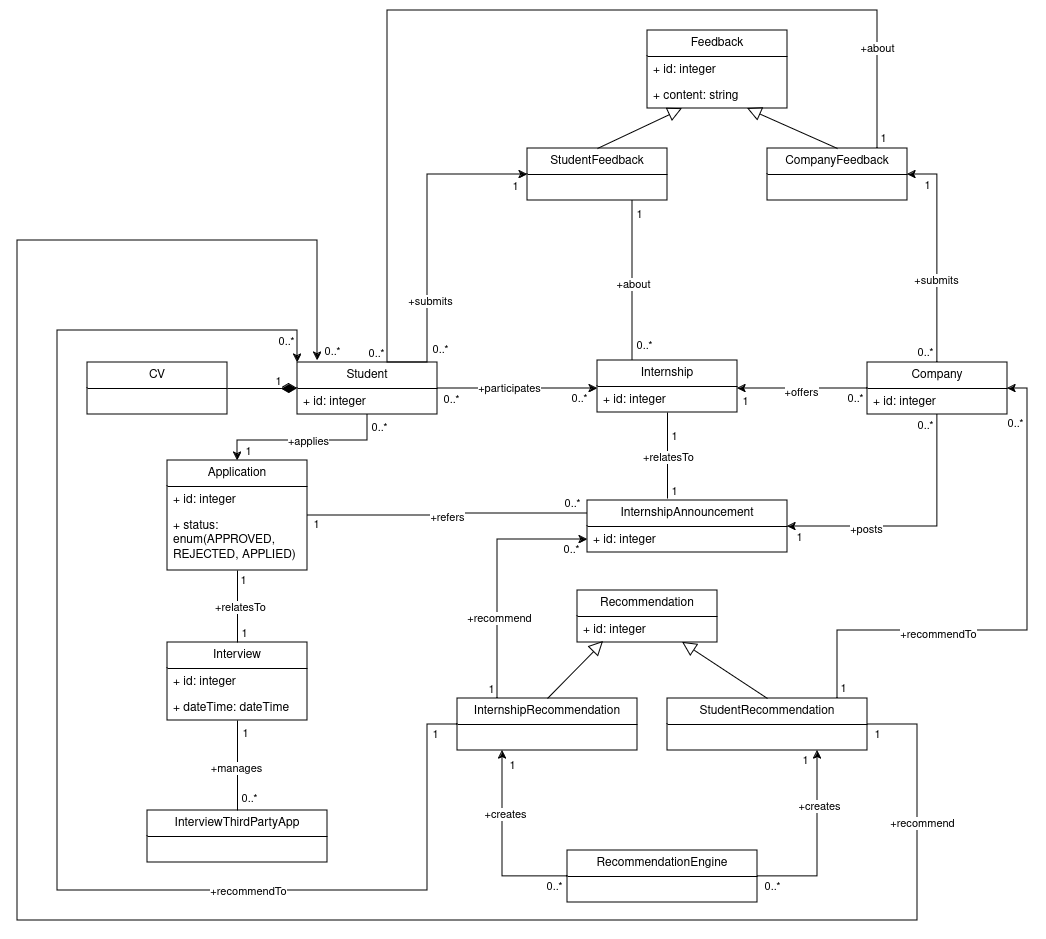
\includegraphics[width=\textwidth]{RASD/images/domain class diagram.png}
\textbf{Domain Class Diagram Description }\newline
The Student class is associated with a single CV, which is the document used to apply for an internship. A Student submits their application in response to an Internship Announcement. Each application has a Status that is initially set to APPLIED. After the company reviews the application, the Status transitions to either APPROVED or REJECTED.
For applications marked as APPROVED, the system facilitates scheduling an interview between the student and the company through a third-party meeting application.
Companies can offer multiple Internships, which are advertised through Internship Announcements. These announcements are the interface where students submit their applications.
The system incorporates a Recommendation Engine that provides two types of recommendations:
\begin{enumerate}
    \item Internship Recommendations: A list of internship opportunities proposed to students based on their profiles and preferences
    \item Student Recommendations: A selection of student profiles proposed to companies based on their requirements and preferences
\end{enumerate}
The system also supports Feedback Mechanisms to enhance transparency and improve future recommendations:
\begin{enumerate}
    \item Student Feedback: After completing an internship, students can provide feedback about the internship experience and the company
    \item Company Feedback: Companies can provide feedback on the performance and professionalism of students who have interned with them
\end{enumerate}

\subsection{State Diagrams }
\textbf{Internship Application}
\newline
\textbf{Application Selection}
\newline
\textbf{Feedback Submission}
\newline

\section{Product functions }

\section{User characteristics }
Two types of users interact with the platform: students and companies
\subsection{Student }
Students can create an account and log in to access the platform, where they can actively search for and apply to internship opportunities or wait to receive personalized notifications for internships that align with their profile. They can also coordinate with companies to schedule interviews through the platform. After completing an internship, students have the opportunity to provide feedback about their experience.
\subsection{Company }
Companies can create an account and log in to access the platform, where they can post detailed internship announcements for students to view and apply to. They can review student applications, approve or reject them as needed, and send notifications to students regarding internships that match their profiles. Companies can also coordinate with students to schedule interviews and provide feedback on the student’s performance after the completion of an internship.

\section{Assumptions, dependencies and constraints }
\subsection{Domain Assumptions }
The following domain assumptions are properties or conditions that the system will take for granted, they must be checked to ensure a correct platform behaviour:
\begin{enumerate}[label={[D\arabic{enumi}]}]
    \item User must have a reliable connection
    \item Students properly insert information about their skills and experiences in their CVs
    \item Companies properly insert information about internships in the announcements
\end{enumerate}

\newpage

\chapter{Specific Requirements }
\label{Specific Requirements}

\section{External Interface Requirements }
\subsection{User Interfaces }
\subsection{Hardware Interfaces }
\subsection{Software Interfaces }
\subsection{Communication Interfaces }

\section{Functional Requirements }
\subsection{Use Cases Diagrams }
\subsection{Use Cases }
\subsection{Sequence Diagrams }
\subsection{Requirements Mapping }

\section{Performance Requirements }

\section{Design Constraints }
\subsection{Standards compliance }
\subsection{Hardware limitations }
\subsection{Any other constraint}

\section{Software System Attributes }
\subsection{Reliability }
\subsection{Availability }
\subsection{Security }
\subsection{Maintainability }
\subsection{Portability }

\newpage

\chapter{Formal Analysis Using Alloy }
\label{Formal Analysis Using Alloy}

\section{Examples }

\newpage

\chapter{Effort Spent }
\label{Effort Spent}

\newpage

\chapter{References}

\newpage
\begin{appendices}
\chapter{Glossary }

\end{appendices}